\documentclass[tikz,border=10pt]{standalone}
\usepackage{tikz}
\usetikzlibrary{positioning,calc,arrows.meta,shadows}
\usepackage{amsmath}

\definecolor{bggray}{RGB}{247,247,249}
\definecolor{titledark}{RGB}{26,35,50}
\definecolor{partyfill}{RGB}{20,74,115}
\definecolor{partyring}{RGB}{163,199,222}
\definecolor{chanfill}{RGB}{229,229,231}
\definecolor{lockblue}{RGB}{20,74,115}
\definecolor{releaseorange}{RGB}{230,126,20}

\begin{document}
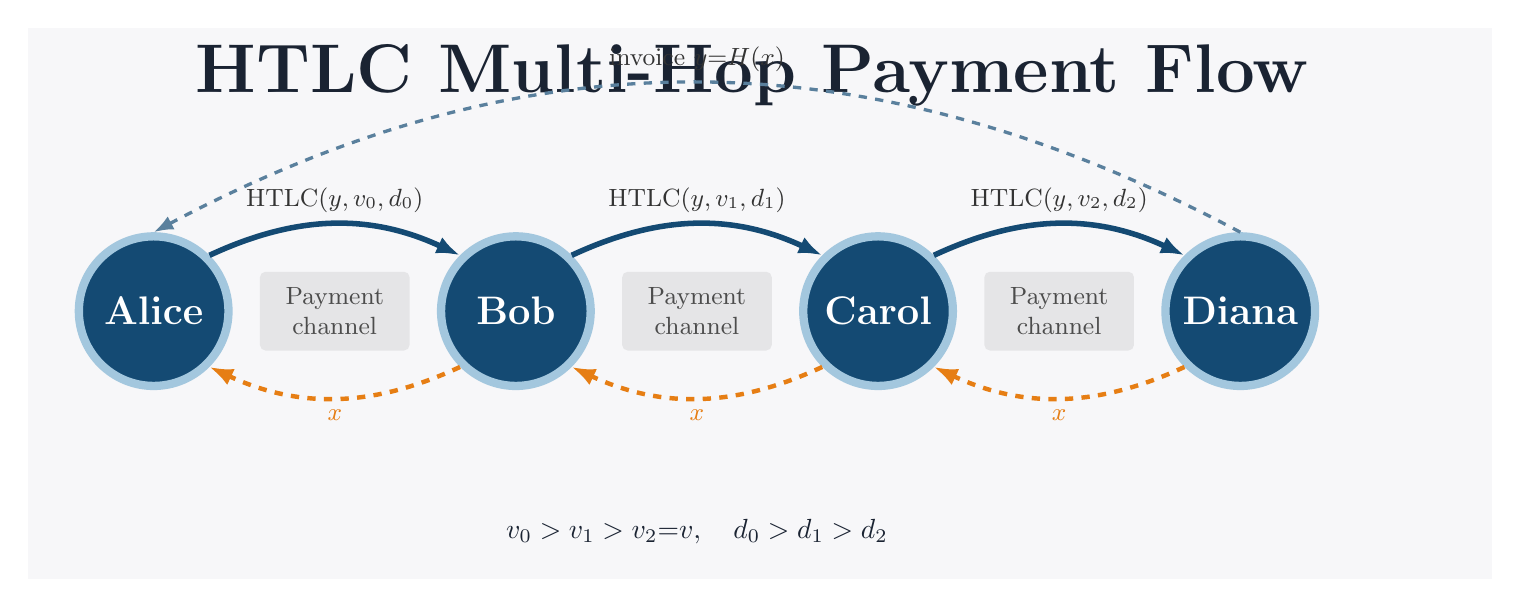
\begin{tikzpicture}[
  x=1cm, y=1cm,
  party/.style={circle, draw=partyring, line width=3pt, fill=partyfill,
                minimum size=1.9cm, font=\Large\bfseries, text=white},
  ch/.style={draw=none, fill=chanfill, rounded corners=2pt,
             minimum width=1.9cm, minimum height=1.0cm,
             font=\small, align=center, text=black!70},
  lockarr/.style={-{Latex[length=3mm]}, line width=2pt, lockblue},
  relarr/.style={-{Latex[length=3mm]}, line width=1.6pt, releaseorange, dashed},
  invarr/.style={-{Latex[length=2.5mm]}, line width=1.2pt, lockblue!70, dashed},
  hoplab/.style={font=\small, text=black!80},
]

% background
\fill[bggray] (-1.6,-3.4) rectangle (17.0,3.6);

% title
\node[font=\Huge\bfseries, titledark] at (7.6,3.0) {HTLC Multi-Hop Payment Flow};

% parties
\node[party] (A) at (0,0)    {Alice};
\node[party] (B) at (4.6,0)  {Bob};
\node[party] (C) at (9.2,0)  {Carol};
\node[party] (D) at (13.8,0) {Diana};

% channel boxes
\node[ch] at ($(A)!0.5!(B)$) {Payment\\channel};
\node[ch] at ($(B)!0.5!(C)$) {Payment\\channel};
\node[ch] at ($(C)!0.5!(D)$) {Payment\\channel};

% invoice arc (top, spans the whole path)
\draw[invarr] (D.north) to[bend right=28]
  node[hoplab, above, pos=0.5] {invoice $y{=}H(x)$} (A.north);

% lock round (solid, curved, above)
\draw[lockarr] (A.north east) to[bend left=25]
  node[hoplab, above, pos=0.5] {HTLC$(y,v_0,d_0)$} (B.north west);
\draw[lockarr] (B.north east) to[bend left=25]
  node[hoplab, above, pos=0.5] {HTLC$(y,v_1,d_1)$} (C.north west);
\draw[lockarr] (C.north east) to[bend left=25]
  node[hoplab, above, pos=0.5] {HTLC$(y,v_2,d_2)$} (D.north west);

% release round (dashed orange, curved, below)
\draw[relarr] (D.south west) to[bend left=25]
  node[hoplab, below, pos=0.5, text=releaseorange] {$x$} (C.south east);
\draw[relarr] (C.south west) to[bend left=25]
  node[hoplab, below, pos=0.5, text=releaseorange] {$x$} (B.south east);
\draw[relarr] (B.south west) to[bend left=25]
  node[hoplab, below, pos=0.5, text=releaseorange] {$x$} (A.south east);

% bottom invariant line
\node[font=\normalsize, titledark] at (6.9,-2.8)
  {$v_0>v_1>v_2{=}v,\quad d_0>d_1>d_2$};

\end{tikzpicture}
\end{document}
